\chapter{Onde elettromagnetiche}

In questo capitolo andremo a dimostrare formalmente come nelle equazioni di Maxwell siano in effetti contenuti fenomeni ondulatori.\\

Prima di far questo è necessario, però, riportare una trattazione matematica delle onde.

\section{Soluzione dell'equazione di d'Alembert}

Un'onda è, nella sua essenza matematica, una perturbazione che si propaga  nello spazio nel corso del tempo mantenendo la propria forma. 
Per formalizzare questo concetto, consideriamo una funzione  $\psi(\mathbf{x}, t)$ che descriva lo stato del campo in ogni punto  dello spazio e in ogni istante di tempo.\\

L'equazione che governa la propagazione di tale perturbazione è l'\emph{equazione di d'Alembert}, o \emph{equazione delle onde}: \mkeyword{equazione di d'Alembert}

\begin{tcolorbox}[colback=yellow!10!white, colframe=orange!70!black, boxrule=0.8pt]
\begin{equation}
    \Box \psi = \frac{1}{v^2}\frac{\partial^2 \psi}{\partial t^2} 
    - \nabla^2 \psi = 0
    \label{eq:dalembert}
\end{equation}
\end{tcolorbox}

dove $v$ è la velocità di propagazione dell'onda e $\Box$ è l'\emph{operatore d'alembertiano}, definito come: \mkeyword{operatore dalembertiano}

\begin{tcolorbox}[colback=yellow!10!white, colframe=orange!70!black, boxrule=0.8pt]
\begin{equation}
    \Box \equiv \nabla^2 - \frac{1}{v^2} \partial_t ^2
\end{equation}
\end{tcolorbox}

L'equazione di d'Alembert è un'equazione alle derivate parziali del secondo ordine, lineare e iperbolica.\\

Nel caso unidimensionale, in cui $\psi = \psi(x, t)$, l'equazione \ref{eq:dalembert} si riduce a:

\begin{equation}
    \frac{\partial^2 \psi}{\partial t^2} - v^2 
    \frac{\partial^2 \psi}{\partial x^2} = 0
    \label{eq:dalembert1d}
\end{equation}

Essa ammette una soluzione generale elegante, ricavabile tramite un opportuno cambio di variabili che diagonalizza l'operatore differenziale, disaccoppiando le direzioni di propagazione.\\

Introduciamo le \textit{coordinate caratteristiche}:

\begin{equation}
    \xi = x - vt, \qquad \eta = x + vt
\end{equation}

e consideriamo $\psi$ come funzione di $\xi$ e $\eta$.  

\newpage

Per la regola della catena, gli operatori di derivazione si trasformano come:

\begin{align}
    \frac{\partial}{\partial x} = \frac{\partial \xi}{\partial x} \frac{\partial}{\partial \xi} + \frac{\partial \eta}{\partial x} \frac{\partial}{\partial \eta} = \frac{\partial}{\partial \xi} + \frac{\partial}{\partial \eta} \\
    \frac{\partial}{\partial t} = \frac{\partial \xi}{\partial t} \frac{\partial}{\partial \xi} + \frac{\partial \eta}{\partial t} \frac{\partial}{\partial \eta} = - v \frac{\partial}{\partial \xi} + v \frac{\partial}{\partial \eta}
\end{align}

da cui, alle derivate seconde:

\begin{align}
    \frac{\partial^2}{\partial x^2} &= \frac{\partial^2}{\partial \xi^2} 
    + 2\frac{\partial^2}{\partial \xi \partial \eta} 
    + \frac{\partial^2}{\partial \eta^2} \\[6pt]
    \frac{\partial^2}{\partial t^2} &= v^2\frac{\partial^2}{\partial \xi^2} 
    - 2v^2\frac{\partial^2}{\partial \xi \partial \eta} 
    + v^2\frac{\partial^2}{\partial \eta^2}
\end{align}

Sostituendo nell'equazione \ref{eq:dalembert1d} e raccogliendo:

\begin{equation}
    v^2\left(\psi_{\xi\xi} - 2\psi_{\xi\eta} + \psi_{\eta\eta}\right)
    - v^2\left(\psi_{\xi\xi} + 2\psi_{\xi\eta} + \psi_{\eta\eta}\right) = 0
\end{equation}

I termini $\psi_{\xi\xi}$ e $\psi_{\eta\eta}$ si cancellano, e l'equazione si riduce alla forma notevolmente semplice:

\begin{equation}
    \frac{\partial^2 \psi}{\partial \xi \, \partial \eta} = 0
    \label{eq:ridotta}
\end{equation}

Questo è il risultato chiave: il cambio di variabili ha \textit{diagonalizzato} l'operatore differenziale, disaccoppiando completamente le due direzioni di propagazione.\\

Procediamo ora con l'integrazione. Dalla \ref{eq:ridotta}, integrando  prima rispetto a $\eta$:

\begin{equation}
    \frac{\partial \psi}{\partial \xi} = f(\xi)
\end{equation}

dove $f(\xi)$ è una funzione arbitraria, poiché la costante di integrazione può dipendere da $\xi$. Integrando nuovamente rispetto a $\xi$:

\begin{equation}
    \psi(\xi, \eta) = F(\xi) + G(\eta)
\end{equation}

dove $F(\xi) = \int f(\xi)\, d\xi$ e $G(\eta)$ sono funzioni arbitrarie di classe $\mathcal{C}^2$. Ritornando alle variabili originali $(x, t)$:

\begin{tcolorbox}[colback=yellow!10!white, colframe=orange!70!black, boxrule=0.8pt]
\begin{equation}
    \psi(x, t) = F(x - vt) + G(x + vt)
\end{equation}
\end{tcolorbox}

La soluzione generale dipende da due funzioni arbitrarie, coerentemente con il fatto che l'equazione \ref{eq:dalembert1d} è del secondo ordine: esse vengono univocamente determinate imponendo le condizioni iniziali $\psi(x, 0)$ e $\partial_t \psi(x, 0)$.

\newpage

\section{Onde elettromagnetiche in assenza di sorgenti nel vuoto e loro proprietà}

Consideriamo innanzitutto il caso dello spazio vuoto, in cui non siano presenti cariche libere e correnti di conduzione, per cui $\rho = 0$ e $\mathbf{j} = 0$. \\

In queste ipotesi le equazioni di Maxwell possono essere riscritte come:

\begin{align*}
    \nabla \cdot \mathbf{E} = 0 \\
    \nabla \cdot \mathbf{B} = 0 \\
    \nabla \times \mathbf{E} = -\dfrac{\partial \mathbf{B}}{\partial t} \\
    \nabla \times \mathbf{B} = \mu_0 \varepsilon_0 \dfrac{\partial \mathbf{E}}{\partial t}
\end{align*}

Queste possono essere disaccoppiate considerando il rotore della legge di Faraday unito alla legge di Ampère-Maxwell

\begin{align*}
    \nabla \times (\nabla \times \mathbf{E}) = \nabla (\nabla \cdot \mathbf{E}) - \nabla^2 \mathbf{E} = \nabla \times \left( - \frac{\partial \mathbf{B}}{\partial t} \right)\\
    = - \frac{\partial}{\partial t} (\nabla \times \mathbf{B}) = - \mu_0 \varepsilon_0 \frac{\partial^2 \mathbf{E}}{\partial t^2}
\end{align*}

E, con un processo analogo per $\mathbf{B}$

\begin{align*}
    \nabla \times (\nabla \times \mathbf{B}) = \nabla (\nabla \cdot \mathbf{B}) - \nabla^2 \mathbf{B} = \nabla \times \left( - \frac{\partial \mathbf{E}}{\partial t} \right)\\
    = - \frac{\partial}{\partial t} (\nabla \times \mathbf{E}) = - \mu_0 \varepsilon_0 \frac{\partial^2 \mathbf{B}}{\partial t^2}
\end{align*}

Dato che $\nabla \cdot \mathbf{E} = 0$ e $\nabla \cdot \mathbf{B} = 0$

\begin{tcolorbox}[colback=yellow!10!white, colframe=orange!70!black, boxrule=0.8pt]
\begin{equation} \label{eq: eq_onda_elettromagnetismo}
    \nabla^2 \mathbf{E} - \mu_0 \varepsilon_0 \frac{\partial^2 \mathbf{E}}{\partial t^2} = 0 \quad , \quad \nabla^2 \mathbf{B} - \mu_0 \varepsilon_0 \frac{\partial^2 \mathbf{B}}{\partial t^2} = 0
\end{equation}
\end{tcolorbox}

Si nota, allora, che $\mathbf{E}$ e $\mathbf{B}$ sono onde che si propagano con velocità 

\begin{tcolorbox}[colback=yellow!10!white, colframe=orange!70!black, boxrule=0.8pt]
\begin{equation}
    c = \frac{1}{\sqrt{\varepsilon_0 \mu_0}}
\end{equation}
\end{tcolorbox}

e se supponiamo che queste si propaghino solo lungo l'asse $x$, per la forma della soluzione dell'equazione di d'Alembert, risulta

\begin{tcolorbox}[colback=yellow!10!white, colframe=orange!70!black, boxrule=0.8pt]
\begin{equation} \label{eq: soluzione_eq_onde_elettromagnetiche}
    \mathbf{E}(x,t) = \mathbf{E}_{-} (x - ct) + \mathbf{E}_{+} (x + ct) \quad , \quad \mathbf{B}(x,t) = \mathbf{B}_{-} (x - ct) + \mathbf{B}_{+} (x + ct)
\end{equation}
\end{tcolorbox}

\subsection{Proprietà delle onde magnetiche nel vuoto}

Dalle equazioni di Maxwell nel vuoto possiamo ricavare altre informazioni oltre alla natura ondulatoria dei campi, infatti limitandoci a cercare una soluzione particolare in cui il campo elettrico $\mathbf{E}$ e il campo magnetico $\mathbf{B}$ dipendano, in un determinato sistema di riferimento cartesiano, solo dal tempo e dalla coordinata $x$ e tenendo conto che nelle nostre ipotesi sono nulle tutte le derivate parziali rispetto a $y$ e $z$, otteniamo:

\begin{align}
\nabla \cdot \mathbf{E} = \frac{\partial E_x}{\partial x} + \frac{\partial E_y}{\partial y} + \frac{\partial E_z}{\partial z} &= 0 & \frac{\partial E_x}{\partial x} &= 0 \\[10pt]
\nabla \cdot \mathbf{B} = \frac{\partial B_x}{\partial x} + \frac{\partial B_y}{\partial y} + \frac{\partial B_z}{\partial z} &= 0 & \frac{\partial B_x}{\partial x} &= 0 \\[10pt]
(\nabla \times \mathbf{E})_x = \frac{\partial E_z}{\partial y} - \frac{\partial E_y}{\partial z} &= -\frac{\partial B_x}{\partial t} & \frac{\partial B_x}{\partial t} &= 0 \\[10pt]
(\nabla \times \mathbf{E})_y = \frac{\partial E_x}{\partial z} - \frac{\partial E_z}{\partial x} &= -\frac{\partial B_y}{\partial t} & \frac{\partial B_y}{\partial t} &= \frac{\partial E_z}{\partial x} \label{eq: 4} \\[10pt] 
(\nabla \times \mathbf{E})_z = \frac{\partial E_y}{\partial x} - \frac{\partial E_x}{\partial y} &= -\frac{\partial B_z}{\partial t} & \frac{\partial B_z}{\partial t} &= -\frac{\partial E_y}{\partial x} \label{eq: 5}\\[10pt]
(\nabla \times \mathbf{B})_x = \frac{\partial B_z}{\partial y} - \frac{\partial B_y}{\partial z} &= \varepsilon_0 \mu_0 \frac{\partial E_x}{\partial t} & \frac{\partial E_x}{\partial t} &= 0 \\[10pt]
(\nabla \times \mathbf{B})_y = \frac{\partial B_x}{\partial z} - \frac{\partial B_z}{\partial x} &= \varepsilon_0 \mu_0 \frac{\partial E_y}{\partial t} & \frac{\partial E_y}{\partial t} &= -\frac{1}{\varepsilon_0 \mu_0}\frac{\partial B_z}{\partial x} \label{eq: 7} \\[10pt]
(\nabla \times \mathbf{B})_z = \frac{\partial B_y}{\partial x} - \frac{\partial B_x}{\partial y} &= \varepsilon_0 \mu_0 \frac{\partial E_z}{\partial t} & \frac{\partial E_z}{\partial t} &= \frac{1}{\varepsilon_0 \mu_0}\frac{\partial B_y}{\partial x} \label{eq: 8}
\end{align}

Le relazioni $\partial E_x/ \partial x = 0$, $\partial E_x/\partial t = 0$ permettono di dedurre che la componente $E_x(x,t)$ del campo elettrico è costante e uniforme e dato che non ci sono sorgenti, $E_x (x,t)= 0$. Allo stesso modo, da $\partial B_x/\partial x = 0$, $\partial B_x/\partial t$ e dall'esclusione di correnti stazionarie concludiamo che $B_x(x,t) = 0$. Questo è un primo risultato importante. \\

Adesso prendiamo in considerazione le \eqref{eq: 4} e \eqref{eq: 5}. Ricordando che nell'ipotesi di propagazione lungo il verso positivo dell'asse delle $x$ le soluzioni della \ref{eq: eq_onda_elettromagnetismo} sono del tipo 

\begin{equation*}
    E_y = E_y(x - ct) \quad , \quad E_z = E_z(x - ct) \quad , \quad B_y = B_y(x - ct) \quad , \quad B_z = B_z(x - ct)
\end{equation*}

Cioè consideriamo solamente la parte progressiva delle \ref{eq: soluzione_eq_onde_elettromagnetiche}. \\

Detto $u = x - ct$ l'argomento delle funzioni, per cui vale $\partial u/ \partial x = 1$ e $\partial u/\partial t = -c$, da \eqref{eq: 4} abbiamo 

\begin{equation}
    \frac{\partial E_z}{\partial x} = \frac{d E_z}{du} \quad , \quad \frac{\partial B_y}{\partial t} = - c \frac{d B_y}{du}
\end{equation}

e quindi 

\begin{equation}
    \frac{d E_z}{du} = - c \frac{d B_y}{du}
\end{equation}

da cui, a meno di una costante di integrazione, che descrive una situazione stazionaria, a cui non siamo interessati,

\begin{equation}
    B_y(x - ct) = - \frac{1}{c} E_y(x - ct) 
\end{equation}

Procedendo analogamente a partire dalla \eqref{eq: 5} si ottiene 

\begin{equation}
    B_z (x - ct) = \frac{1}{c} E_y(x - ct)
\end{equation}

Le componenti del campo $\mathbf{B}$ risultato pertanto dipendenti da quelle del campo $\mathbf{E}$ e i due vettori si possono scrivere nella forma 

\begin{tcolorbox}[colback=yellow!10!white, colframe=orange!70!black, boxrule=0.8pt]
\begin{align}
    \mathbf{E}(x,t) = E_y(x - ct) \mathbf{u}_y + E_z(x - ct)\mathbf{u}_z\\
    c \mathbf{B}(x,t) = - E_z(x - ct) \mathbf{u}_y + E_y(x - ct) \mathbf{u}_z
\end{align}
\end{tcolorbox}

Da questa relazione si ricava che tra i moduli dei campi, in ogni istante e in ogni punto 

\begin{tcolorbox}[colback=yellow!10!white, colframe=orange!70!black, boxrule=0.8pt]
\begin{equation}
    B = \frac{E}{c} \quad , \quad E = cB \quad , \quad \frac{E}{B} = c
\end{equation}
\end{tcolorbox}

Mentre dal prodotto scalare si ottiene 

\begin{tcolorbox}[colback=yellow!10!white, colframe=orange!70!black, boxrule=0.8pt]
\begin{equation}
    \mathbf{E} \cdot \mathbf{B} = E_y B_y + E_z B_z = \frac{1}{c} (-E_y E_z + E_z E_y) = 0
\end{equation}
\end{tcolorbox}

Pertanto $\mathbf{E}$ e $\mathbf{B}$ \emph{sono sempre ortogonali tra loro}. \\

Invece il prodotto vettoriale vale 

\begin{tcolorbox}[colback=yellow!10!white, colframe=orange!70!black, boxrule=0.8pt]
\begin{equation}
    \mathbf{E} \times \mathbf{B} = \frac{E^2}{c} \mathbf{u}_x = c B^2 \mathbf{u}_x = E B \mathbf{u}_x
\end{equation}
\end{tcolorbox}

\newpage

\section{Onde monocromatiche nel vuoto}

Supponiamo, come sopra, di essere nel vuoto e in assenza di sorgenti, in modo che tutti i risultati trovati in questo capitolo fino ad ora siano ancora validi. Tuttavia adesso diamo una forma particolare alla soluzione 

\begin{tcolorbox}[colback=yellow!10!white, colframe=orange!70!black, boxrule=0.8pt]
\begin{align}
    \mathbf{E}(x, t) = \Re[\mathbf{E}_0 e^{i(k(x - c t))}] = \Re[\mathbf{E}_0 e^{i(kx - \omega t)}] \\
    \mathbf{B}(x, t) = \Re[\mathbf{B}_0 e^{i(k(x - c t))}] = \Re[\mathbf{B}_0 e^{i(kx - \omega t)}] 
\end{align}
\end{tcolorbox}

Dove $\mathbf{E}_0$ e $\mathbf{B}_0$ sono le ampiezze (complesse) e abbiamo posto 

\begin{tcolorbox}[colback=yellow!10!white, colframe=orange!70!black, boxrule=0.8pt]
\begin{equation}
    \omega = k c
\end{equation}
\end{tcolorbox}

Tuttavia il versore $\mathbf{u}_x$ non ha alcuna particolarità, possiamo scegliere un generico versore $\mathbf{u}_n$ come direzione per la propagazione dell'onda. Quindi si ha 

\begin{tcolorbox}[colback=yellow!10!white, colframe=orange!70!black, boxrule=0.8pt]
\begin{align}
    \mathbf{E}(\mathbf{r}, t) = \Re[\mathbf{E}_0 e^{i(\mathbf{k} \cdot \mathbf{r} - \omega t)}] \\
    \mathbf{B}(\mathbf{r}, t) = \Re[\mathbf{B}_0 e^{i(\mathbf{k} \cdot \mathbf{r} - \omega t)}] 
\end{align}
\end{tcolorbox}

Dove abbiamo posto $\mathbf{k} = k \ \mathbf{u}_n$, quindi $\mathbf{k}$ è il vettore che ha modulo pari al numero d'onda $k$ \mkeyword{numero d'onda} e direzione e verso della propagazione dell'onda.\\

\begin{figure}[h]
    \centering
    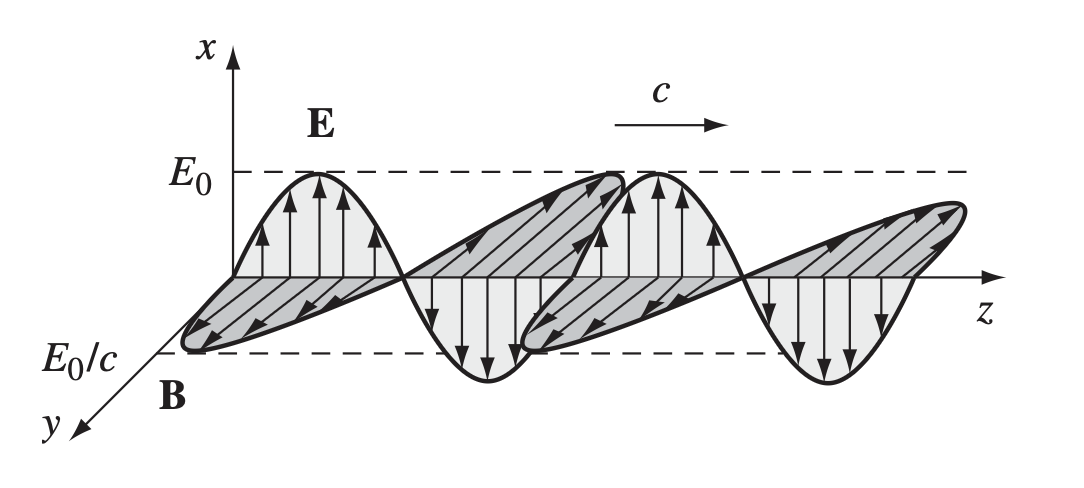
\includegraphics[width=0.8\textwidth]{figure/image66.png}
    \caption{Onda monocromatica}
    \label{fig:}
\end{figure}


Dalle relazione precedenti si ha 

\begin{tcolorbox}[colback=yellow!10!white, colframe=orange!70!black, boxrule=0.8pt]
\begin{equation}
    \mathbf{E}_0 \cdot \mathbf{k} = 0 \quad , \quad \mathbf{B}_0 \cdot \mathbf{k} = 0
\end{equation}
\end{tcolorbox}

\newpage

Inoltre conoscendo una delle due ampiezze complesse e la propagazione dell'onda è possibile ricavare anche l'altra ampiezza complessa.

\begin{tcolorbox}[colback=yellow!10!white, colframe=orange!70!black, boxrule=0.8pt]
\begin{align}
    \mathbf{E}_0 = c (\mathbf{B}_0 \times \mathbf{u}_n) \\
    \mathbf{B}_0 = \frac{1}{c} (\mathbf{u}_n \times \mathbf{E}_0)
\end{align}
\end{tcolorbox}

O analogamente, in termini di $\mathbf{k}$

\begin{tcolorbox}[colback=yellow!10!white, colframe=orange!70!black, boxrule=0.8pt]
\begin{align}
    \mathbf{E}_0 = \frac{\omega}{c^2} (\mathbf{B}_0 \times \mathbf{k}) \\
    \mathbf{B}_0 = \frac{1}{\omega} (\mathbf{k} \times \mathbf{E}_0)
\end{align}
\end{tcolorbox}

Chiaramente l’onda piana è di fatto un’astrazione matematica in quanto non esiste una sorgente fisica infinitamente estesa nello spazio che la possa produrre. Le sorgenti reali hanno un’estensione finita e questo che fa sì che la soluzione dell’equazione delle onde elettromagnetiche possa essere molto complicata.
Tuttavia, per quanto possano essere complessi, fronti d’onda non planari possono essere comunque localmente approssimati con il piano tangente.

\subsection{Polarizzazione delle onde elettromagnetiche monocromatiche}

\newpage

\subsection{Energia di un'onda elettromagnetica monocromatica}

Dalla \ref{eq: densità_totale_energia} sappiamo che l'energia per unità di volume di un campo elettromagnetico è 

\begin{equation}
    u = \frac{1}{2} \left(\varepsilon_0 E^2 + \frac{1}{\mu_0}B^2\right)
\end{equation}

Nel caso dell'onda monocromatica si ha 

\begin{equation}
    B^2 = \frac{1}{c^2} E^2 = \mu_0 \varepsilon_0 E^2
\end{equation}

quindi il campo elettrico e magnetico danno lo stesso contributo

\begin{tcolorbox}[colback=yellow!10!white, colframe=orange!70!black, boxrule=0.8pt]
\begin{equation}
    u = \varepsilon_0 E^2 = \varepsilon_0 E_0^2 \cos^2(kx - \omega t)
\end{equation}
\end{tcolorbox}

Il flusso di energia (per unità di area e di tempo) trasportato dal campo è dato dal vettore di Poynting \eqref{eq: vettore_Poynting}

\begin{equation}
    \mathbf{S} = \frac{1}{\mu_0} (\mathbf{E} \times \mathbf{B})
\end{equation}

Allora, per lo stesso motivo di prima

\begin{tcolorbox}[colback=yellow!10!white, colframe=orange!70!black, boxrule=0.8pt]
\begin{equation}
    \mathbf{S} = c \varepsilon_0 E_0^2 \cos^2(kx - \omega t) \ \mathbf{u}_n = c u \ \mathbf{u}_n
\end{equation}
\end{tcolorbox}

Si nota che $\mathbf{S}$ è la densità di energia moltiplicata per la velocità dell'onda, in accordo con il teorema di Poynting \eqref{eq: teorema_di_Poynting}.

Tipicamente, però, non siamo interessati al vettore di Poyting o alla densità di energia in ogni istante, ma al loro \emph{valor medio}. La media del coseno quadro lungo un periodo completo è $\frac{1}{2}$, quindi 

\begin{tcolorbox}[colback=yellow!10!white, colframe=orange!70!black, boxrule=0.8pt]
\begin{align}
    \langle u \rangle = \frac{1}{2}\varepsilon_0 E_0^2 \\
    \langle \mathbf{S} \rangle = \frac{1}{2} c \varepsilon_0 E_0^2 \ \mathbf{u}_n
\end{align}
\end{tcolorbox}

La potenza media per unità di area trasportata da un'onda elettromagnetica è chiamata intensità: \mkeyword{intesità}

\begin{tcolorbox}[colback=yellow!10!white, colframe=orange!70!black, boxrule=0.8pt]
\begin{equation}
    I \equiv \langle S \rangle = \frac{1}{2} c \varepsilon_0 E_0^2
\end{equation}
\end{tcolorbox}

\newpage

\section{Onde sferiche nel vuoto}

Un caso altrettanto semplice dal punto di vista analitico (quanto irrealistico dal punto di vista fisico), è rappresentato dall'onda sferica. \\


\begin{figure}[h]
  \centering
  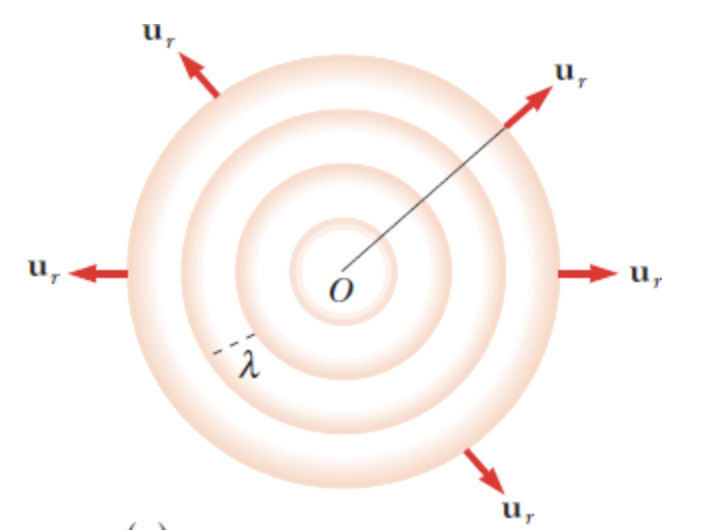
\includegraphics[width=0.4\linewidth]{figure/image67.png}
  \label{fig:etichetta}
\end{figure}

\'E opportuno, allora, tornare all'equazione generale delle onde scalari nello spazio tridimensionale 

\begin{equation}
    \nabla^2 \psi - \frac{1}{v^2} \frac{\partial^2 \psi}{\partial t^2}  
\end{equation}

dove la funzione d'onda dipende dalla posizione e dal tempo. 
Supponiamo che il problema abbia simmetria sferica, allora, tenendo conto dell'operato laplaciano in coordinate sferiche e della simmetria del problema, l'equazione precedente diventa

\begin{equation}
    \frac{1}{r} \frac{\partial^2 (r \psi)}{\partial r^2} = \frac{1}{v^2} \frac{\partial^2(\psi)}{\partial t^2}
\end{equation}

che è equivalente a 

\begin{equation}
    \frac{\partial^2 (r \psi)}{\partial r^2} = \frac{1}{v^2} \frac{\partial^2(r \psi)}{\partial t^2}
\end{equation}


Da un punto di vista strettamente matematico questa espressione è del tutto analoga all'equazione di d'Alembert per la funzione $r \psi$. Allora possiamo \emph{scegliere} come soluzione 

\begin{equation}
\psi(r,t) = \frac{A_{-} e^{i(kr - \omega t)}}{r} + \frac{A_{+} e^{i(kr + \omega t)}}{r}
\end{equation}

Limitando il nostro interesse ad onde armoniche esplosive, prodotte da una sorgente puntiforme con emissione isotropa (simmetria sferica) si ha che 

\begin{tcolorbox}[colback=yellow!10!white, colframe=orange!70!black, boxrule=0.8pt]
\begin{equation}
    \psi(r,t) = A \frac{e^{i(\mathbf{k}\cdot \mathbf{r} - \omega t)}}{r}
\end{equation}
\end{tcolorbox}

Poiché le equazioni di Maxwell nel vuoto, in assenza di sorgenti, si riducono a equazioni d'onda disaccoppiate per ciascuna componente dei campi $\mathbf{E}$ e $\mathbf{B}$, la soluzione trovata per $\psi$ può essere identificata con una qualsiasi componente cartesiana di questi campi. 
Tuttavia, non tutte le combinazioni sono fisicamente ammissibili: $\mathbf{E}$ e $\mathbf{B}$ devono soddisfare simultaneamente le equazioni di Maxwell, il che impone vincoli aggiuntivi - in particolare che i campi siano trasversali alla direzione di propagazione $\mathbf{u}_n$ e mutuamente ortogonali.

\newpage

\section{Onde cilindriche nel vuoto}

Un altro tipo di onde particolarmente importanti sono le onde cilindriche. \\

Tuttavia prima di trattare in dettaglio questo tipo di onde è necessario introdurre uno strumento matematico che ci servirà in seguito. 

\subsection{Funzioni di Bessel}

In coordinate cilindriche $(\rho, \phi, z)$ l'equazione di Laplace assume la forma 

\begin{equation}
    \frac{\partial^2 \psi}{\partial \rho^2} + \frac{1}{\rho} \frac{\partial \psi}{\partial \rho} + \frac{1}{\rho^2} \frac{\partial^2 \psi}{\partial \phi^2} + \frac{\partial^2 \psi}{\partial z^2} = 0
\end{equation}

La separazione delle variabili si ottiene con la sostituzione 

\begin{equation}
    \psi(\rho, \phi, z) = R(\rho) Q(\phi) Z(z)
\end{equation}

Questo conduce alle tre equazioni differenziali ordinarie:

\begin{align}
    \frac{d^2 Z}{dz^2} - k^2 Z = 0 \\
    \frac{d^2 Q}{d \phi^2} + \nu^2 Q = 0 \\
    \frac{d^2 R}{d \rho^2} + \frac{1}{\rho} \frac{dR}{d\rho} + \left( k^2 - \frac{\nu^2}{\rho^2} \right) R = 0
\end{align}

Le soluzioni alle prime due equazioni si ricavano facilmente:

\begin{align}
    Z(z) = e^{\pm kz}\\
    Q(\phi) = e^{\pm \nu \phi}
\end{align}

L'equazione radiale di può porre in una forma standard con il cambio di variabile $x = k\rho$. Essa diventa allora 

\begin{tcolorbox}[colback=yellow!10!white, colframe=orange!70!black, boxrule=0.8pt]
\begin{equation} \label{eq: equazione_Bessel}
    \frac{d^2 R}{dx^2} + \frac{1}{x} \frac{dR}{dx} + \left( 1 - \frac{\nu^2}{x^2} \right) R = 0
\end{equation}
\end{tcolorbox}

Questa è l'equazione di Bessel, \mkeyword{equazione di Bessel}e le sue soluzioni sono chiamate funzioni di Bessel di ordine $\nu$.\\

Se si assume un'equazione in serie di potenze del tipo 

\begin{equation}
    R(x) = x^{\alpha} \sum_{j = 0}^{\infty} a_j x^{j}
\end{equation}

sostituendo si ottiene che 

\begin{equation}
    \alpha = \pm \nu
\end{equation}

e 

\begin{equation}
    a_{2j} = - \frac{1}{4j (j + \alpha)} a_{2j-2}
\end{equation}

Tutte le potenze dispari di $x^j$ hanno coefficienti nulli. La formula di ricorrenza può essere iterata per dare 

\begin{equation}
a_{2 j}=\frac{(-1)^j \Gamma(\alpha+1)}{2^{2 j} j!\Gamma(j+\alpha+1)} a_0
\end{equation}

\'E conveniente porre la costante $a_0 = [2^\alpha \Gamma(\alpha +1)]^{-1}$. Le due soluzioni sono allora 

\begin{tcolorbox}[colback=yellow!10!white, colframe=orange!70!black, boxrule=0.8pt]
\begin{equation}
\begin{aligned}
J_\nu(x) & =\left(\frac{x}{2}\right)^\nu \sum_{j=0}^{\infty} \frac{(-1)^j}{j!\Gamma(j+\nu+1)}\left(\frac{x}{2}\right)^{2 j} \\
J_{-\nu}(x) & =\left(\frac{x}{2}\right)^{-\nu} \sum_{j=0}^{\infty} \frac{(-1)^j}{j!\Gamma(j-\nu+1)}\left(\frac{x}{2}\right)^{2 j}
\end{aligned}
\end{equation}
\end{tcolorbox}

Queste soluzioni sono chiamate funzioni di Bessel del primo tipo e di ordine $\pm \nu$. \mkeyword{funzioni di Bessel del primo tipo}

Se $\nu$ \emph{non} è intero, queste due soluzioni $J_{\pm \nu} (x)$ formano una coppia di soluzioni linearmente indipendenti. Tuttavia se $\nu$ è intero è ben noto che le soluzioni sono linearmente dipendenti. \\
In effetti, per $\nu = m$ intero, si può vedere dalla rappresentazione in serie che 

\begin{equation}
    J_{-m}(x) = (-1)^m J_m(x)
\end{equation}

Di conseguenza quando $\nu$ è intero è necessario trovare un'altra soluzione linearmente indipendente. Anche quando $\nu$ non è un intero è comune sostituire la coppia $j_{\pm}(x)$ con $J_{\nu}(x)$ e $N_{\nu} (x)$, quest'ultima è detta funzione di Neumann (o funzione di Bessel del secondo tipo) e vale: \mkeyword{funzione di Bessel del secondo tipo}

\begin{tcolorbox}[colback=yellow!10!white, colframe=orange!70!black, boxrule=0.8pt]
\begin{equation}
    N_{\nu} = \frac{J_{\nu}(x) \cos{\nu \pi} - J_{-\nu} (x)}{\sin{\nu \pi}}
\end{equation}
\end{tcolorbox}

Esistono anche le funzioni di Bessel del terzo\mkeyword{funzioni di Bessel del terzo tipo} tipo\footnote{per un approfondimento su questo argomento si consigli di guarda il capitolo 3.7 del \cite{ElettrodinamicaClassica}} che prendono il nome di funzioni di Hankel e sono le seguenti combinazioni lineari di $J_{\nu}(x)$ e $N_{\nu}(x)$:

\begin{tcolorbox}[colback=yellow!10!white, colframe=orange!70!black, boxrule=0.8pt]
\begin{equation}
\begin{array}{l}
H_\nu^{(1)}(x)=J_\nu(x)+i N_\nu(x) \\
H_\nu^{(2)}(x)=J_\nu(x)-i N_\nu(x)
\end{array}
\end{equation}
\end{tcolorbox}

\newpage

Particolarmente interessanti sono le forme asintotiche delle funzioni di Bessel per valori molto grandi e molto piccolo dei loro argomenti. \\

Se supponiamo $x \ll 1$:

\begin{tcolorbox}[colback=yellow!10!white, colframe=orange!70!black, boxrule=0.8pt]
\begin{align}
J_{\nu}(x) \rightarrow \frac{1}{\Gamma(\nu+1)}\left(\frac{x}{2}\right)^{\nu}\\
N_{\nu}(x) \rightarrow
\begin{cases}
  \dfrac{2}{\pi}\left[\ln\left(\frac{x}{2}\right) + 0{,}5772\cdots\right], & \nu = 0 \\[10pt]
  -\dfrac{\Gamma(\nu)}{\pi}\left(\frac{2}{x}\right)^{\nu}, & \nu \neq 0
\end{cases}
\end{align}
\end{tcolorbox}

Se supponiamo $x \gg 1$:

\begin{tcolorbox}[colback=yellow!10!white, colframe=orange!70!black, boxrule=0.8pt]
\begin{align}
    J_{\nu}(x) \rightarrow \sqrt{\frac{2}{\pi x}}\cos\left(x - \frac{\nu\pi}{2} - \frac{\pi}{4}\right)\\
    N_{\nu}(x) \rightarrow \sqrt{\frac{2}{\pi x}}\sin\left(x - \frac{\nu\pi}{2} - \frac{\pi}{4}\right)
\end{align}
\end{tcolorbox}

Adesso possiamo passare alla formulazione formale delle onde cilindriche.\\

\begin{figure}[h]
  \centering
  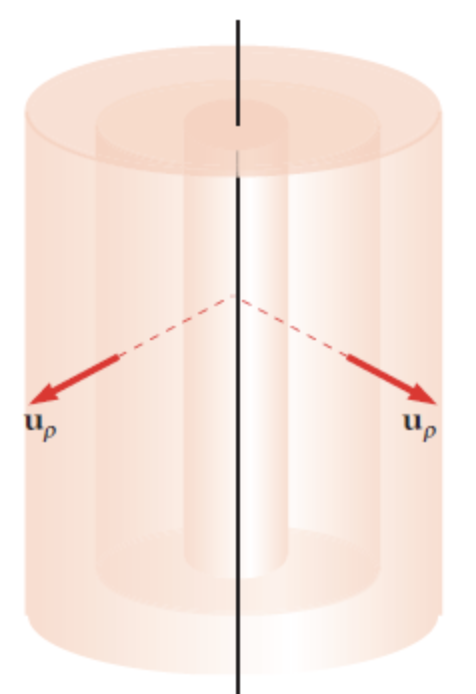
\includegraphics[width=0.3\linewidth]{figure/image68.png}
  \caption{Onda cilindrica}
  \label{fig:etichetta}
\end{figure}

Per descriverle conviene usare un sistema di coordinate cilindriche con l'asse $z$ coincidente con la retta sorgente. Supponendo che le coordinate del campo elettrico e magnetico dipendano solo da $\rho$, per ciascuna componente dei campi vale 

\begin{equation}
    \frac{1}{\rho} \frac{\partial \psi}{\partial \rho} + \frac{\partial^2 \psi}{\partial \rho^2} = \frac{1}{v^2} \frac{\partial^2 \psi}{\partial t^2}
\end{equation}

Procedendo per separazione delle variabili, ed assumendo dipendenza temporale armonica semplice, si pone 

\begin{equation}
    \psi(\rho,t) = R(\rho) e^{-i \omega t}
\end{equation}

in cui la parte spaziale $R(\rho)$ deve essere soluzione di 

\begin{equation}
    \rho \frac{d^2 R}{d \rho^2} + \frac{dR}{d\rho} - k^2 \rho R = 0
\end{equation}

La quale è la funzione di Bessel \eqref{eq: equazione_Bessel} dove $x = k\rho$ e si ha che $\nu = 0$. Pertanto, dato che siamo nel caso in cui $\nu$ è intero, si ha che la soluzione è 

\begin{equation}
        R(\rho) = A J_{0}(k\rho) + B N_{0} (k\rho)
\end{equation}

Dove $A$ e $B$ sono due costanti di integrazione. \\

Se supponiamo di essere nel caso $k \rho \gg 1$ si ha che 

\begin{tcolorbox}[colback=yellow!10!white, colframe=orange!70!black, boxrule=0.8pt]
\begin{equation}
    J_0(k \rho) \approx \sqrt{\frac{2}{\pi k \rho}} \cos \left(k \rho - \frac{\pi}{4}\right) \quad , \quad N_{0}(k \rho) \approx \sqrt{\frac{2}{\pi k \rho}} \sin\left(k \rho - \frac{\pi}{4}\right)
\end{equation}
\end{tcolorbox}

Quindi, in questo limite 

\begin{tcolorbox}[colback=yellow!10!white, colframe=orange!70!black, boxrule=0.8pt]
\begin{equation}
\psi (\rho, t) = \frac{A_p}{\sqrt{\rho}} e^{i(k\rho - \omega t)} + \frac{A_r}{\sqrt{\rho}} e^{i(k \rho + \omega t)}
\end{equation}
\end{tcolorbox}

La parte della soluzione con $J_0$ è legata ad onde convergenti, quella con $N_0$ alle onde divergenti. Quanto detto vale per onde scalari, che si propagano nella direzione del versore $\mathbf{u}_{\rho}$

\newpage

\section{Onde elettromagnetiche in assenza di sorgenti in un mezzo}

Supponiamo di essere in un mezzo, ma in una regione in cui non siano presenti cariche libere e correnti di conduzione, per cui $\rho = 0$ e $\mathbf{j} = 0$. 

In queste ipotesi le equazioni di Maxwell possono essere scritte come 

\begin{align*}
    \nabla \cdot \mathbf{D} = 0 \\
    \nabla \cdot \mathbf{B} = 0 \\
    \nabla \times \mathbf{E} = -\dfrac{\partial \mathbf{B}}{\partial t} \\
    \nabla \times \mathbf{H} = \dfrac{\partial \mathbf{D}}{\partial t}
\end{align*}

Se il mezzo è lineare:

\begin{equation}
    \mathbf{D} = \varepsilon \mathbf{E} \quad , \quad \mathbf{H} = \frac{1}{\mu} \mathbf{B}
\end{equation}

e omogeneo (in modo che $\eps$ e $\mu$ non varino nello spazio), le equazioni si riducono a 

\begin{align*}
    \nabla \cdot \mathbf{E} = 0 \\
    \nabla \cdot \mathbf{B} = 0 \\
    \nabla \times \mathbf{E} = -\dfrac{\partial \mathbf{B}}{\partial t} \\
    \nabla \times \mathbf{B} = \mu \varepsilon \dfrac{\partial \mathbf{E}}{\partial t}
\end{align*}

che differiscono con l'analogo corrispondente nel vuoto solo per il termine $\eps \mu$. \\

\emph{Pertanto tutti i risultati ottenuti in precedenza sono ancora validi, cambia solamente che al posto di $c$ dobbiamo mettere $v$, dove}

\begin{tcolorbox}[colback=yellow!10!white, colframe=orange!70!black, boxrule=0.8pt]
\begin{equation}
    v = \frac{1}{\sqrt{\eps \mu}} = \frac{c}{n} 
\end{equation}
\end{tcolorbox}

dove 

\begin{tcolorbox}[colback=yellow!10!white, colframe=orange!70!black, boxrule=0.8pt]
\begin{equation}
    n = \sqrt{\frac{\eps \mu}{\eps_0 \mu_0}}
\end{equation}
\end{tcolorbox}

è l'indice di rifrazione della sostanza. \mkeyword{indice di rifrazione}Per la maggior parte dei materiali, il valore di $\mu$ è molto vicino a quello di $\mu_0$, quindi

\begin{equation}
    n \approx\sqrt{\kappa_e}
\end{equation}

\subsection{Onde monocromatiche in un mezzo}

Anche i risultati per le onde monocromatiche continuano a essere validi, è però interessante vedere come cambia la densità di energia e il vettore di Poynting. \\

La densità di energia risulta essere 

\begin{equation}
    u = \frac{1}{2} \left( \eps E^2 + \frac{1}{\mu} B^2 \right)
\end{equation}

e il vettore di Poynting è 

\begin{equation}
    \mathbf{S} = \frac{1}{\mu} (\mathbf{E} \times \mathbf{B})
\end{equation}

In particolare, per le onde monocromatiche piane, per quanto visto prima, vale 

\begin{tcolorbox}[colback=yellow!10!white, colframe=orange!70!black, boxrule=0.8pt]
\begin{equation}
    I = \frac{1}{2} \eps v E_0^2 = \frac{1}{2} \frac{n}{Z_0} E_0^2
\end{equation}
\end{tcolorbox}

dove abbiamo posto 

\begin{tcolorbox}[colback=yellow!10!white, colframe=orange!70!black, boxrule=0.8pt]
\begin{equation}
    Z_0 = \sqrt{\frac{\mu_0}{\eps_0}} \approx 377 \Omega
\end{equation}
\end{tcolorbox}

Questa quantità prende il nome di impedenza nel vuoto. \mkeyword{impedenza nel vuoto}

\newpage

\section{Soluzione equazione d'onda con sorgente}

Consideriamo adesso il caso generale delle equazioni di Maxwell, cioè il caso in cui siano presenti anche delle sorgenti.\\

Osservando le equazioni di Maxwell in forma potenziale in gauge di Lorenz \ref{eq: Gauge_Lorenz}, si nota che le equazioni sono tutte nella stessa forma, cioè

\begin{tcolorbox}[colback=yellow!10!white, colframe=orange!70!black, boxrule=0.8pt]
\begin{equation}\label{eq: equazione_onda_non_omogenea}
    \nabla^2 \psi - \frac{1}{c^2} \frac{\partial^2 \psi}{\partial t^2} = -4 \pi f(\mathbf{r},t)
\end{equation}
\end{tcolorbox}

Dove il termine $-4 \pi$ è stato aggiunto per un motivo che sarà chiaro tra poco. \\

Andiamo a trovare una soluzione generale a questa equazione.\\

Possiamo considerare una generica sorgente $f(\mathbf{r}, t)$ come una sovrapposizione di sorgenti puntiformi

\begin{equation}
    f(\mathbf{r}, t) = \int \int f(\mathbf{r'}, t') \delta(\mathbf{r} - \mathbf{r'}) \delta(t - t') d^3 r' dt'
\end{equation}

ma allora si intuisce che $\psi$ dovrà essere nella forma 

\begin{equation}
    \psi (\mathbf{r}, t) = \int \int G(\mathbf{r},\mathbf{r'}, t, t') f (\mathbf{r'}, t') d^3 r' dt'
\end{equation}

Dove $G(\mathbf{r},\mathbf{r'}, t, t')$ è la funzione di Green associata all'operatore dalembertiano, cioè la funzione che soddisfa la relazione 

\begin{equation}
    \Box^2 G(\mathbf{r}, \mathbf{r'}, t, t') = - 4 \pi \delta(\mathbf{r} - \mathbf{r'}) \delta(t -t')
\end{equation}

Pertanto, sostituendo, la \ref{eq: equazione_onda_non_omogenea} si riduce a 

\begin{tcolorbox}[colback=yellow!10!white, colframe=orange!70!black, boxrule=0.8pt]
\begin{equation} \label{eq: equazione_onda_non_omogena_Green}
    (\nabla^2 - \frac{1}{c^2} \partial_t^2) G(\mathbf{r}, \mathbf{r'}, t, t') = -4 \pi \delta(\mathbf{r} - \mathbf{r'})\delta (t - t') 
\end{equation}
\end{tcolorbox}

Inoltre sappiamo che possiamo esprimere la delta secondo la trasformata di Fourier come 

\begin{equation}
    \delta(t - t') = \frac{1}{2\pi} \int_{-\infty}^{\infty} e^{-i \omega (t-t')} d\omega
\end{equation}

Poiché la sorgente è una sovrapposizione di termini $e^{-i\omega t}$, per linearità dell'equazione cerchiamo $G(\mathbf{r}, \mathbf{r'}, t, t')$ della stessa forma:

\begin{tcolorbox}[colback=yellow!10!white, colframe=orange!70!black, boxrule=0.8pt]
\begin{equation} \label{eq: legame_Green_tempo_spazio}
    G(\mathbf{r}, \mathbf{r'}, t, t') = \frac{1}{2\pi} \int_{-\infty}^{\infty} \tilde{G}_{\omega}(\mathbf{r}, \mathbf{r'}) \cdot e^{-i \omega (t -t')} d\omega
\end{equation}
\end{tcolorbox}

Dove $\tilde{G}_{\omega}$ rappresenta la parte spaziale da determinare. 

\newpage

Applicando il dalembertiano al nostro ansatz si ha:

\begin{align}
    \nabla^2 G = \frac{1}{2\pi} \int_{-\infty} \nabla^2 \tilde{G}_{\omega} \cdot e^{-i \omega (t-t')} d\omega\\
    -\frac{1}{c^2} \frac{\partial^2}{\partial t^2} G = \frac{1}{2\pi} \int_{-\infty}^{\infty} \frac{\omega^2}{c^2} \tilde{G}_{\omega} \cdot e^{-i \omega (t - t')} d \omega
\end{align}

Allora raccogliendo tutto la \ref{eq: equazione_onda_non_omogena_Green} diventa 

\begin{equation}
\frac{1}{2\pi} \int_{-\infty}^{\infty} \left( \nabla^2 + \frac{\omega^2}{c^2} \right) \tilde{G}_{\omega} \cdot e^{-i\omega (t-t')} d\omega = \frac{1}{2\pi} \int_{-\infty}^{\infty} \left( -4\pi \delta(\mathbf{r} - \mathbf{r'}) \right) \cdot e^{-i\omega (t-t')} d\omega
\end{equation}

Poiché questo deve valere per ogni $\omega$, i termini sotto l'integrale devono essere uguali frequenza per frequenza:

\begin{tcolorbox}[colback=yellow!10!white, colframe=orange!70!black, boxrule=0.8pt]
\begin{equation}\label{eq: equazione_Helmholtz}
    \left( \nabla^2 + \frac{\omega^2}{c^2} \right) \tilde{G}_{\omega} = - 4\pi \delta(\mathbf{r} - \mathbf{r'})
\end{equation}
\end{tcolorbox}

Ci siamo quindi ricondotti a un nuovo tipo di equazione che prende il nome di equazione di Helmholtz. \mkeyword{equazione di Helmholtz}

\subsection{Soluzione equazione di Helmholtz}

Poniamo $k = \frac{\omega}{c}$, allora la \ref{eq: equazione_Helmholtz} diventa

\begin{equation}
    (\nabla^2 + k^2) \tilde{G}_{\omega} (\mathbf{r}, \mathbf{r'}) = -4\pi \delta(\mathbf{r} - \mathbf{r'})
\end{equation}

Allora si nota che $\tilde{G}_{\omega}$ non è altro che la funzione di Green associata all'operatore $(\nabla^2 + k^2)$.\\

Se non vi sono superfici di confine, la funzione di Green può dipendere soltanto da $\mathbf{R} = \mathbf{r} - \mathbf{r'}$, e deve essere a simmetria sferica, ossia deve dipendere soltato da $R = |\mathbf{R}|$. Dalla forma dell'operatore laplaciano in coordinate sferiche è chiaro che $\tilde{G}_{\omega}(R)$ soddisfa 

\begin{equation}
    \frac{1}{R}\frac{d^2}{dR^2} (R \tilde{G}_{\omega}) + k^2 \tilde{G}_{\omega} = -4 \pi\delta(R) 
\end{equation}

Dato che stiamo considerano un'equazione con una delta, $R \tilde{G}_{\omega}(R)$ soddisfa in tutto lo spazio tranne che in $R = 0$ l'equazione omogenea 

\begin{equation}
    \frac{d^2}{dR^2} (R \tilde{G}_{\omega}) + k^2 (R \tilde{G}_{\omega}) = 0
\end{equation}

con soluzione 

\begin{equation}
    R \tilde{G}_{\omega}(R) = A e^{ikR} + B e^{-ikR}
\end{equation}

Mentre quando $R \to 0$ siamo vicini alla sorgente puntuale e in questo limite $kR \ll 1$, il che significa che il termine $k^2$ nell'equazione di Helmholtz diventa trascurabile rispetto a $\nabla^2$, e l'equazione si riduce a quella di Poisson:

\begin{equation}
    \nabla^2 \tilde{G}_{\omega} \approx -4\pi \delta(R)
\end{equation}

Dall'equazione di Poisson sappiamo già che la soluzione è il potenziale columbiano: 

\begin{equation}
    \tilde{G}_{\omega}(R) \xrightarrow{R \to 0} \frac{1}{R}
\end{equation}

Questo fissa la normalizzazione. Guardando la soluzione generale:

\begin{equation*}
    R \tilde{G}_{\omega}(R) = A e^{ikR} + B e^{-ikR}
\end{equation*}

Per $R \to 0$ si ha che $e^{\pm i kR} \to 1$, quindi:

\begin{equation*}
    R \tilde{G}_{\omega}(R) \to A + B \implies \tilde{G}_{\omega}(R) \xrightarrow{R \to 0} \frac{A + B}{R}
\end{equation*}

Affinché questo coincida con $1/R$, bisogna imporra:

\begin{equation}
    A + B = 1
\end{equation}

Questo è il vincolo che fissa la normalizzazione della soluzione generale. \\

Pertanto si ha che la soluzione generale dell'equazione di Helmholtz è 

\begin{tcolorbox}[colback=yellow!10!white, colframe=orange!70!black, boxrule=0.8pt]
\begin{align} 
    \tilde{G}_{\omega}(R) = A \tilde{G}_{\omega}^{(+)}(R) + B \tilde{G}_{\omega}^{(-)}(R) \\
    A + B = 1
\end{align}
\end{tcolorbox}

Dove abbiamo definito 

\begin{tcolorbox}[colback=yellow!10!white, colframe=orange!70!black, boxrule=0.8pt]
\begin{align} 
    \tilde{G}_{\omega}^{(\pm)}(R) = \frac{e^{\pm i k R}}{R} 
\end{align}
\end{tcolorbox}

Allora possiamo andare a sostituire questo risultato nella \ref{eq: legame_Green_tempo_spazio} e ottenere

\begin{equation}
    G^{(\pm)} (R, \tau) = \frac{1}{2\pi} \int_{-\infty}^{+\infty} \frac{e^{\pm ikR}}{R} \cdot e^{-i\omega \tau} \ d\omega
\end{equation}

Dove abbiamo posto $\tau = t - t'$. Si nota che questo integrale è una delta e quindi le funzioni di Green sono 

\begin{equation}
    G^{(\pm)}(R, \tau) = \frac{1}{R} \delta(\tau \mp \frac{R}{c}) 
\end{equation}

oppure, più esplicitamente

\begin{tcolorbox}[colback=yellow!10!white, colframe=orange!70!black, boxrule=0.8pt]
\begin{equation}
    G^{(\pm)}(\mathbf{r}, \mathbf{r'}, t, t') = \frac{\delta \left(t' - \left[ t \mp \frac{|\mathbf{r} - \mathbf{r}'|}{c} \right] \right)}{|\mathbf{r} - \mathbf{r'}|}
\end{equation}
\end{tcolorbox}

La funzione di Green $G^{(+)}$ è chiamata \emph{funzione di Green ritardata} \mkeyword{funzione di Green ritardata} perché esibisce il comportamento causale associato ad una perturbazione ondulatoria.
L'argomento della funziona delta mostra che un effetto osservato nel punto $\mathbf{r}$ all'istante $t$ è causato dall'azione di una sorgente a distanza $R$ in un istante precendete o ritardato $t' = t - R/c$. La differenza temporale $R/c$ è semplicemente il tempo di propagazione della perturbazione da un punto all'altro. \\

Analogamente, $G^{(-)}$ è chiamata \emph{funzione di Green anticipata}. \mkeyword{funzione di Green anticipata}\\

Gli integrali particolari dell'equazione d'onda non omogenea sono

\begin{equation}
    \psi^{(\pm)}(\mathbf{r}, t) = \int \int G^{(\pm)}(\mathbf{r}, \mathbf{r'}, t, t') f(\mathbf{r'}, t') \, d^3r' \, dt'
\end{equation}

Per determinare un problema fisico assegnato, può essere necessario aggiungere ad entrambe queste soluzioni una soluzione dell'equazione omogenea. Consideriamo una distribuzione di sorgenti $f(\mathbf{r'}, t')$ che sia localizzata nello spazio e nel tempo. Essa è diversa da zero solo per un intervallo temporale limitato attorno a $t' = 0$. Si possono identificare due situazioni limite. \\

Nella prima si assume che per $t \to -\infty$ vi sia un'onda $\psi_{\text{in}}$ che soddisfa l'equazione d'onda omogenea. Questa onda si propaga nel tempo e nello spazio; la sorgente si accende e genera le sue proprie onde. La soluzione completa a tutti i tempi per questa situazione è chiaramente

\begin{equation}
    \psi(\mathbf{r}, t) = \psi_{\text{in}}(\mathbf{r}, t) + \int \int G^{(+)}(\mathbf{r}, \mathbf{r'}, t, t') f(\mathbf{r'}, t') \, d^3r' \, dt'
\end{equation}

La presenza di $G^{(+)}$ assicura che nel lontano passato, prima che la sorgente venga attivata, non vi sono contributi all'integrale. È presente soltanto l'onda assegnata $\psi_{\text{in}}$. \\

La seconda situazione è quella per cui a tempi lontani nel futuro ($t \to +\infty$) venga assegnata l'onda $\psi_{\text{out}}$, una soluzione nota dell'equazione d'onda omogenea. La soluzione completa a tutti i tempi è allora

\begin{equation}
    \psi(\mathbf{r}, t) = \psi_{\text{out}}(\mathbf{r}, t) + \int \int G^{(-)}(\mathbf{r}, \mathbf{r'}, t, t') f(\mathbf{r'}, t') \, d^3r' \, dt'
\end{equation}

La funzione di Green anticipata garantisce ora l'assenza di qualsiasi segnale dalla sorgente una volta che questa sia stata spenta (tali segnali sono per definizione contenuti in $\psi_{\text{out}}$). \\

La situazione fisica più comune è descritta dall'equazione precedente con $\psi_{\text{in}} = 0$. Essa viene a volte scritta sostituendo esplicitamente la funzione di Green:

\begin{tcolorbox}[colback=yellow!10!white, colframe=orange!70!black, boxrule=0.8pt]
\begin{equation} \label{eq: soluzioni_ritardate}
    \psi(\mathbf{r}, t) = \int \frac{\left[ f(\mathbf{r'}, t') \right]_{\text{rit}}}{|\mathbf{r} - \mathbf{r'}|} \, d^3r'
\end{equation}
\end{tcolorbox}

La parentesi quadra $[\cdots]_{\text{rit}}$ significa che il tempo $t'$ deve essere calcolato all'istante ritardato $t' = t - |\mathbf{r} - \mathbf{r'}|/c$.

\section{Potenziali ritardati}

Utilizzando le soluzioni ritardate \ref{eq: soluzioni_ritardate} per le equazioni d'onda \ref{eq: Gauge_Lorenz} si ottiene 

\begin{tcolorbox}[colback=yellow!10!white, colframe=orange!70!black, boxrule=0.8pt]
\begin{align} \label{potenziali ritardati}
    \phi(\mathbf{r},t) = \frac{1}{4\pi \eps_0} \int_{\tau} \frac{[\rho (\mathbf{r'}, t')]_{\text{rit}}}{|\mathbf{r} - \mathbf{r'}|} d^3r' = \frac{1}{4\pi \eps_0} \int_{\tau} \frac{\rho (\mathbf{r'}, t - \frac{|\mathbf{r} - \mathbf{r}'|}{c})}{|\mathbf{r} - \mathbf{r'}|} d^3r'\\
    \mathbf{A}(\mathbf{r},t) = \frac{\mu_0}{4\pi} \int_{\tau} \frac{[\mathbf{j}(\mathbf{r}', t')]_{\text{rit}}}{|\mathbf{r} - \mathbf{r'}|} d^3 r' = \frac{\mu_0}{4\pi} \int_{\tau} \frac{\mathbf{j}(\mathbf{r}', t - \frac{|\mathbf{r} - \mathbf{r}'|}{c})}{|\mathbf{r} - \mathbf{r'}|} d^3 r' 
\end{align}
\end{tcolorbox}

I potenziali ritardati \ref{potenziali ritardati} sono la generalizzazione dinamica dei potenziali statici di Coulomb e Biot-Savart: la distribuzione di carica e corrente che contribuisce al potenziale nel punto $\mathbf{r}$ all'istante $t$ non è quella presente in $\mathbf{r'}$ all'istante $t$, bensì quella presente all'istante ritardato $t' = t - |\mathbf{r} - \mathbf{r'}|/c$, cioè il tempo necessario affinché un segnale che viaggia alla velocità della luce raggiunga $\mathbf{r}$ da $\mathbf{r'}$.\\

Questo risultato è fisicamente fondamentale: i campi elettromagnetici non si propagano istantaneamente, ma con velocità $c$, in accordo con la causalità relativistica. \footnote{\'E possibile ottenere anche un'espressione esplicita per i campi grazie all'equazione di Jefimenko, tuttavia l'utilità di questi è limitata dato che solitamente è più semplice calcolare i potenziali ritardati e differenziarli se necessario. 
Si trovano approfondimenti in \cite{ElettrodinamicaClassica} e \cite{IntroductiontoElectrodynamics}}

\subsection{Potenziali di Liénard-Wiechert}

Un caso particolarmente importante e istruttivo è quello di una carica puntiforme $q$ in moto con traiettoria $\mathbf{r}_q(t)$ e velocità  $\mathbf{v}(t) = \dot{\mathbf{r}}_q(t)$. Le distribuzioni di carica e corrente sono:

\begin{align}
    \rho(\mathbf{r'}, t') = q \, \delta(\mathbf{r'} - \mathbf{r}_q(t')) \\
    \mathbf{j}(\mathbf{r'}, t') = q \, \mathbf{v}(t') \delta(\mathbf{r'} - \mathbf{r}_q(t'))
\end{align}

Sostituendo nelle \ref{potenziali ritardati} e integrando con attenzione — tenendo conto che la delta temporale introduce un fattore geometrico dovuto alla dipendenza di $|\mathbf{r} - \mathbf{r'}|$ dalla posizione della carica — si ottengono i \emph{potenziali di Liénard-Wiechert}: \mkeyword{potenziali di Liénard-Wiechert}

\begin{tcolorbox}[colback=yellow!10!white, colframe=orange!70!black, boxrule=0.8pt]
\begin{align} \label{eq: potenziali_Liènard-Wiechert}
    \phi(\mathbf{r}, t) = \frac{q}{4\pi\varepsilon_0} \left( \frac{1}{\mathcal{R} - \boldsymbol{\mathcal{R}} \cdot \boldsymbol{\beta}} \right)_{\text{rit}} \\
    \mathbf{A}(\mathbf{r}, t) = \frac{\mu_0 q c}{4\pi} \left( \frac{\boldsymbol{\beta}}{\mathcal{R} - \boldsymbol{\mathcal{R}} \cdot \boldsymbol{\beta}} \right)_{\text{rit}}
\end{align}
\end{tcolorbox}

dove abbiamo definito:

\begin{align}
    \boldsymbol{\mathcal{R}} = \mathbf{r} - \mathbf{r}_q(t') \quad &, \quad \mathcal{R} = |\boldsymbol{\mathcal{R}}| \\
    \boldsymbol{\beta} = \frac{\mathbf{v}(t')}{c} \quad &, \quad \beta = |\boldsymbol{\beta}|
\end{align}

tutti valutati all'istante ritardato $t'$. Il fattore $(1 - \hat{\mathcal{R}} \cdot \boldsymbol{\beta})$ al denominatore è una conseguenza geometrica della propagazione finita del segnale: una carica che si avvicina all'osservatore con velocità prossima a $c$ produce un campo molto più intenso rispetto al caso statico, mentre una carica che si allontana lo produce più debole — un effetto analogo all'effetto Doppler relativistico.

Si noti inoltre la relazione semplice tra i due potenziali:

\begin{tcolorbox}[colback=yellow!10!white, colframe=orange!70!black, 
boxrule=0.8pt]
\begin{equation}
    \mathbf{A}(\mathbf{r}, t) = \frac{\boldsymbol{\beta}_{\text{rit}}}{c} 
    \phi(\mathbf{r}, t)
\end{equation}
\end{tcolorbox}

\section{Sorgenti monocromatiche e sviluppo in multipoli}

Consideriamo sorgenti con dipendenza temporale armonica, ovvero 

\begin{equation}
    \rho(\mathbf{r'}, t) = \rho(\mathbf{r'}) e^{-i\omega t} \quad , \quad 
    \mathbf{j}(\mathbf{r'}, t) = \mathbf{j}(\mathbf{r'}) e^{-i\omega t}
\end{equation}

Per linearità delle equazioni, anche i potenziali avranno la stessa dipendenza temporale:

\begin{equation}
    \phi(\mathbf{r}, t) = \phi(\mathbf{r}) e^{-i\omega t} \quad , \quad 
    \mathbf{A}(\mathbf{r}, t) = \mathbf{A}(\mathbf{r}) e^{-i\omega t}
\end{equation}

Sostituendo nei potenziali ritardati \ref{potenziali ritardati}, il tempo ritardato $t_r = t - |\mathbf{r} - \mathbf{r'}|/c$ introduce un fattore di fase $e^{ik|\mathbf{r}-\mathbf{r'}|}$, con $k = \omega/c$, e le parti spaziali dei potenziali diventano:

\begin{tcolorbox}[colback=yellow!10!white, colframe=orange!70!black, 
boxrule=0.8pt]
\begin{align}
    \phi(\mathbf{r}) = \frac{1}{4\pi\varepsilon_0} \int 
    \rho(\mathbf{r'}) \frac{e^{ik|\mathbf{r}-\mathbf{r'}|}}
    {|\mathbf{r}-\mathbf{r'}|} \, d^3r' \\[6pt]
    \mathbf{A}(\mathbf{r}) = \frac{\mu_0}{4\pi} \int 
    \mathbf{j}(\mathbf{r'}) \frac{e^{ik|\mathbf{r}-\mathbf{r'}|}}
    {|\mathbf{r}-\mathbf{r'}|} \, d^3r'
\end{align}
\end{tcolorbox}

Il nucleo comune a entrambi gli integrali è la funzione di Green dell'operatore di Helmholtz:

\begin{equation}
    G(\mathbf{r}, \mathbf{r'}) = \frac{e^{ik|\mathbf{r}-\mathbf{r'}|}}
    {|\mathbf{r}-\mathbf{r'}|}
\end{equation}

Supponiamo ora che la sorgente sia confinata in un volume di dimensione tipica $d$, e cerchiamo i campi a distanza $r = |\mathbf{r}| \gg d$. 
In questa ipotesi è possibile espandere $G$ in potenze di $r'/r \ll 1$.\\

Partendo dall'identità geometrica esatta

\begin{equation}
    |\mathbf{r} - \mathbf{r'}| = r\sqrt{1 - 2\frac{\hat{r}\cdot\mathbf{r'}}{r} 
    + \frac{r'^2}{r^2}} \approx r - \hat{r}\cdot\mathbf{r'}
\end{equation}

\newpage

valida al primo ordine in $r'/r$, si ottiene:

\begin{equation}
    G(\mathbf{r}, \mathbf{r'}) \approx \frac{e^{ikr}}{r} \, 
    e^{-ik\hat{r}\cdot\mathbf{r'}}
\end{equation}

dove abbiamo approssimato $1/|\mathbf{r}-\mathbf{r'}| \approx 1/r$ nell'ampiezza (lecito per $r \gg d$) ma mantenuto la correzione $e^{-ik\hat{r}\cdot\mathbf{r'}}$ nella fase, poiché anche piccole variazioni di fase possono avere effetti significativi.\\

Espandendo infine l'esponenziale in serie:

\begin{tcolorbox}[colback=yellow!10!white, colframe=orange!70!black, boxrule=0.8pt]
\begin{equation} \label{eq: sviluppo_multipoli_ritard}
    e^{-ik\hat{r}\cdot\mathbf{r'}} = \sum_{n=0}^{\infty} 
    \frac{(-ik)^n}{n!} (\hat{r}\cdot\mathbf{r'})^n 
    = 1 - ik(\hat{r}\cdot\mathbf{r'}) + \cdots
\end{equation}
\end{tcolorbox}

Il primo termine ($n=0$) corrisponde all'approssimazione di dipolo elettrico, in cui il tempo ritardato è lo stesso per tutta la sorgente e non dipende da $\mathbf{r'}$. In altre parole, questa è l'approssimazione in cui stiamo considerando la sorgente come un oggetto puntiforme che oscilla come un unico dipolo.

\subsection{Le tre zone}

Prima di procedere con il calcolo esplicito dei campi, è utile identificare tre regioni dello spazio con caratteristiche fisiche distinte, determinate dal confronto tra $r$, $d$ e la lunghezza d'onda $\lambda = 2\pi/k$:

\begin{itemize}
    \item \textbf{Zona quasi-statica} (campo prossimo): $d \ll r \ll \lambda$, 
    ovvero $kr \ll 1$. In questo regime $e^{ikr}/r \approx 1/r$ e i campi 
    hanno la stessa struttura dei campi statici, con una dipendenza 
    temporale $e^{-i\omega t}$.

    \item \textbf{Zona di induzione} (campo intermedio): $d \ll r \sim \lambda$, 
    ovvero $kr \sim 1$. I termini di velocità e di accelerazione sono 
    comparabili, e la struttura dei campi è più complicata. Questa zona 
    è rilevante per esempio nelle antenne in campo vicino.

    \item \textbf{Zona di radiazione} (campo lontano): $d \ll \lambda \ll r$, 
    ovvero $kr \gg 1$. Dominano i termini che decadono come $1/r$, 
    responsabili del trasporto netto di energia. Questa è la zona 
    fisicamente più importante per lo studio dell'irraggiamento.
\end{itemize}

\newpage

\section{Dipolo elettrico oscillante}

Consideriamo una distribuzione di cariche e correnti monocromatica confinata in un volume piccolo ($d \ll \lambda$). Nell'approssimazione di dipolo \emph{elettrico} ($n=0$ nello sviluppo precedente) il potenziale vettore è:

\begin{equation}
    \mathbf{A}_0(\mathbf{r}) = \frac{\mu_0}{4\pi} \frac{e^{ikr}}{r} 
    \int \mathbf{j}(\mathbf{r'}) \, d^3r'
\end{equation}

L'integrale della densità di corrente è collegato alla derivata temporale del momento di dipolo elettrico. Utilizzando l'equazione di continuità $\nabla \cdot \mathbf{j} = -\partial_t \rho = i\omega\rho$ e integrando per parti, si dimostra che:

\begin{equation}
    \int \mathbf{j}(\mathbf{r'}) \, d^3r' = -\int \mathbf{r}' (\nabla' \cdot \mathbf{j}) = -i\omega \int \mathbf{r}' \rho(\mathbf{r}') \ d^3 r' = -i\omega \mathbf{p}_0
\end{equation}

dove $\mathbf{p}_0 = \int \rho(\mathbf{r'}) \mathbf{r'} \, d^3r'$ è l'ampiezza del momento di dipolo elettrico. Definendo il momento di dipolo come $\mathbf{p}(t) = \mathbf{p}_0 e^{-i\omega t}$ e al tempo ritardato $\mathbf{p}_r = \mathbf{p}(t - r/c)$, il potenziale vettore completo risulta:

\begin{tcolorbox}[colback=yellow!10!white, colframe=orange!70!black,boxrule=0.8pt]
\begin{equation}\label{eq: potenziale_vettore_dipolo}
    \mathbf{A}_0(\mathbf{r}, t) = \frac{\mu_0}{4\pi} 
    \frac{\dot{\mathbf{p}}_r}{r}
\end{equation}
\end{tcolorbox}

Il potenziale scalare si ricava dalla gauge di Lorenz $\nabla \cdot \mathbf{A} = -\frac{1}{c^2}\partial_t \phi$:

\begin{tcolorbox}[colback=yellow!10!white, colframe=orange!70!black, boxrule=0.8pt]
\begin{equation}
    \phi_0(\mathbf{r}, t) = \frac{1}{4\pi\varepsilon_0} 
    \frac{(\mathbf{p}_r + \frac{r}{c}\dot{\mathbf{p}}_r)\cdot\hat{r}}{r^2}
\end{equation}
\end{tcolorbox}

\subsection{Campi del dipolo elettrico oscillante}

A partire dai potenziali si ricavano i campi $\mathbf{B} = \nabla \times \mathbf{A}$ e $\mathbf{E} = -\nabla\phi - \partial_t \mathbf{A}$. 
Definendo $\mathbf{p}^* = \mathbf{p}_r + \frac{r}{c}\dot{\mathbf{p}}_r$, il risultato completo è:

\begin{tcolorbox}[colback=yellow!10!white, colframe=orange!70!black, 
boxrule=0.8pt]
\begin{align}
    \mathbf{B} &= \frac{\mu_0}{4\pi} 
    \frac{\mathbf{p}^* \times \hat{r}}{r^2} 
    \sim \frac{\dot{\mathbf{p}}_r}{r^2} = \frac{\ddot{\mathbf{p}}_r}{r} 
    \label{eq: B_dipolo}\\[8pt]
    \mathbf{E} &= \frac{1}{4\pi\varepsilon_0} \left[ 
    \frac{3(\mathbf{p}^*\cdot\hat{r})\hat{r} - \mathbf{p}^*}{r^3} 
    + \frac{1}{c^2} 
    \frac{(\ddot{\mathbf{p}}_r \times \hat{r}) \times \hat{r}}{r}
    \right] \label{eq: E_dipolo}
\end{align}
\end{tcolorbox}

I campi si separano naturalmente in due contributi con andamenti diversi in $r$:

\begin{itemize}
    \item \textbf{Campo prossimo} ($r \ll \lambda$): dominano i termini 
    $\sim r^{-3}$ e $\sim r^{-2}$. Sviluppando il tempo ritardato 
    $\mathbf{p}_r = \mathbf{p}(t) - \frac{r}{c}\dot{\mathbf{p}}(t) + \cdots$ 
    si verifica che $\mathbf{p}^* \to \mathbf{p}(t)$, e il campo elettrico 
    si riduce a quello di un dipolo statico istantaneo:
    \begin{equation}
        \mathbf{E} \approx \frac{1}{4\pi\varepsilon_0} 
        \frac{3(\mathbf{p}(t)\cdot\hat{r})\hat{r} - \mathbf{p}(t)}{r^3}
    \end{equation}
    Il campo magnetico $\mathbf{B} \sim \dot{\mathbf{p}}/r^2$ corrisponde 
    alla legge di Biot-Savart per correnti variabili nel tempo.

\newpage

    \item \textbf{Campo di radiazione} ($r \gg \lambda$): domina il termine $\sim r^{-1}$, che decade lentamente e trasporta energia a grande distanza. I campi risultano:

    \begin{tcolorbox}[colback=yellow!10!white, colframe=orange!70!black, boxrule=0.8pt]
    \begin{align}
        \mathbf{E}_{\text{rad}} &= \frac{1}{4\pi\varepsilon_0 c^2} 
        \frac{(\ddot{\mathbf{p}}_r \times \hat{r}) \times \hat{r}}{r} 
        \label{eq: E_rad_dipolo}\\[6pt]
        \mathbf{B}_{\text{rad}} &= \frac{\mu_0}{4\pi c} 
        \frac{\ddot{\mathbf{p}}_r \times \hat{r}}{r}
        \label{eq: B_rad_dipolo}
    \end{align}
    \end{tcolorbox}

    Si nota che $\mathbf{E}_{\text{rad}}$ è proporzionale alla componente di $\ddot{\mathbf{p}}_r$ \emph{trasversale} a $\hat{r}$, e che $\frac{1}{c}\mathbf{E}_{\text{rad}} = \mathbf{B}_{\text{rad}} \times \hat{r}$: i due campi sono mutuamente ortogonali e ortogonali alla direzione di propagazione $\hat{r}$, esattamente come per un'onda piana. 
    Se $\hat{r} \parallel \ddot{\mathbf{p}}_r$ i campi si annullano.\\

    Quindi, ad esempio, se il dipolo oscilla lungo $\hat{z}$, $\mathbf{B}_{\text{rad}}$ avrà componente solo lungo $\hat{\phi}$, mentre $\mathbf{E}_{\text{rad}}$ avrà componente solo lungo $\hat{\theta}$.
\end{itemize}

\begin{figure}[h]
  \centering
  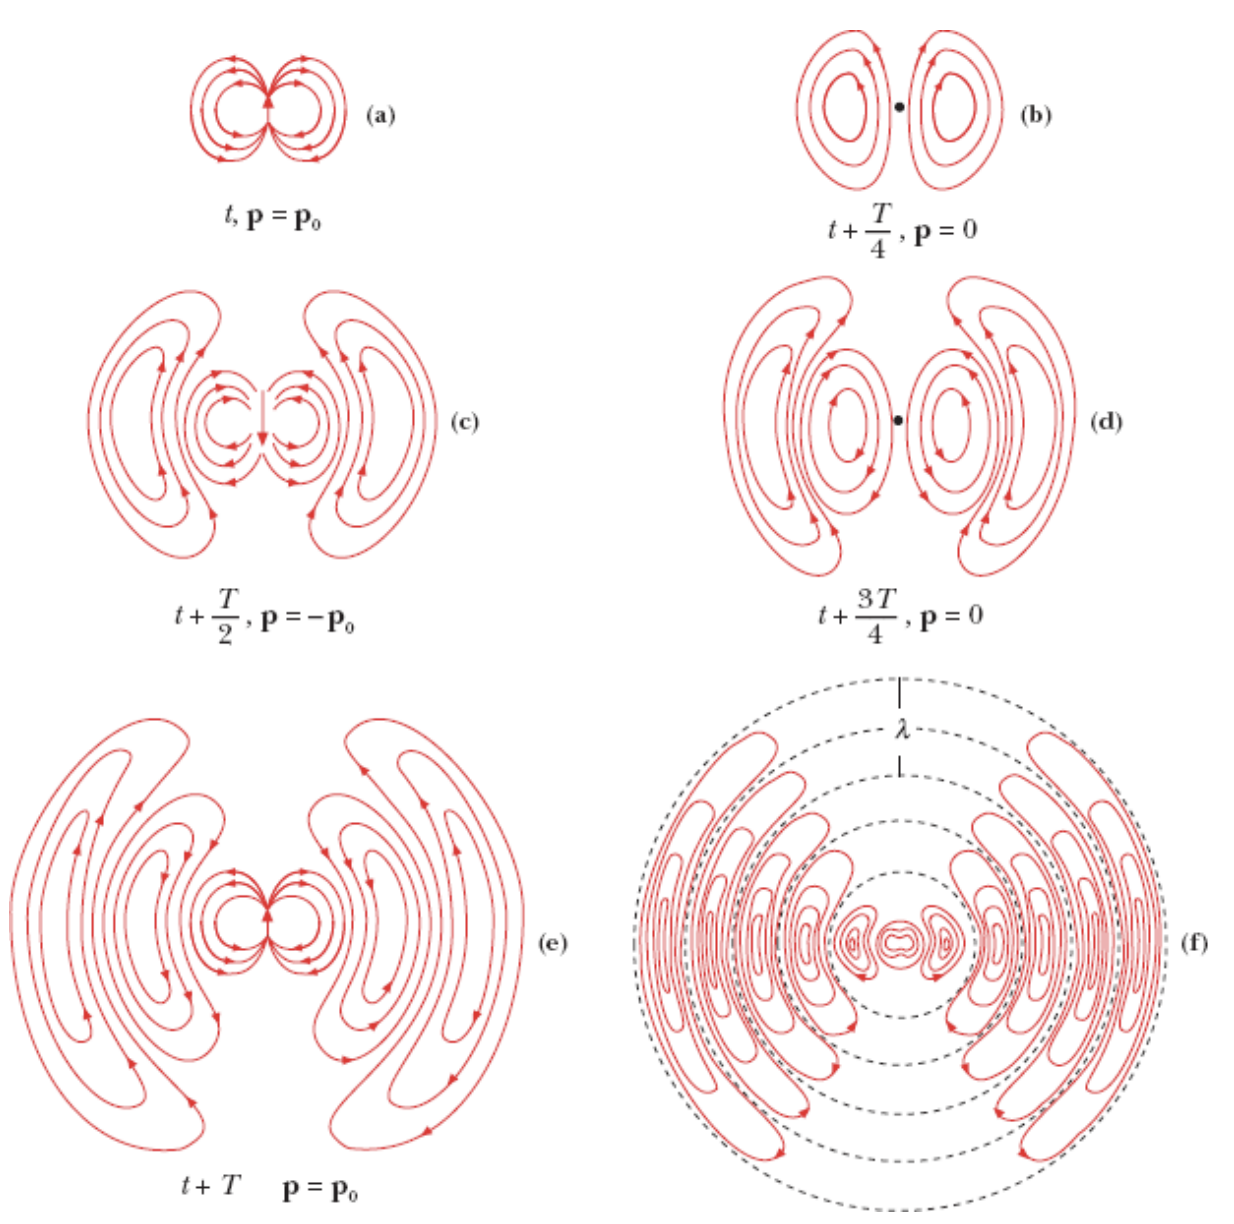
\includegraphics[width=0.65\linewidth]{figure/image69.png}
  \caption{Rappresentazione schematica della produzione e della propagazione delle linee di campo elettrico prodotte da un dipolo elettrico oscillante}
  \label{fig:etichetta}
\end{figure}

\newpage

\section{Termine di ordine successivo: dipolo magnetico e quadrupolo elettrico}

Come prima consideriamo una distribuzione di cariche e correnti monocromatica confinata in un volume piccolo ($d \ll \lambda$), ma ora includiamo il termine $n=1$ nello sviluppo \eqref{eq: sviluppo_multipoli_ritard}.
Il contributo di questo termine al potenziale vettore è 

\begin{equation}
    \mathbf{A}_1(\mathbf{r}) = \frac{\mu_0}{4 \pi} \frac{e^{ik}}{r} (-ikr) \int (\hat{r} \cdot \mathbf{r}')\mathbf{j}(\mathbf{r}') \ d^3 r'
\end{equation}

Includendo la dipendenza temporale e ricordando che $-ik = -i\omega/c = \partial_t/c$, si ha:

\begin{equation}
    \mathbf{A}_1(\mathbf{r}, t) = \frac{\mu_0}{4\pi c} \frac{\partial_t}{r} \int(\hat{r} \cdot \mathbf{r}') \mathbf{j} (\mathbf{r}', t_r) \ d^3 r'  
\end{equation}

\footnote{Attenzione, in questi appunti la notazione $t_r$, $[t']_{\text{rit}}$ hanno lo stesso significato, cioè indicano entrambe il tempo ritardato.} Per andare a semplificare l'integrale, scomponiamo l'integrando in parte simmetrica e antisimmetrica rispetto allo scambio $\hat{r} \leftrightarrow \mathbf{j}$:

\begin{align}
    (\hat{r} \cdot \mathbf{r'}) \mathbf{j} = \frac{1}{2}\left[(\hat{r} \cdot \mathbf{r'}) \mathbf{j} + (\hat{r} \cdot \mathbf{j}) \mathbf{r'}\right] + \frac{1}{2}\left[(\hat{r} \cdot \mathbf{r'}) \mathbf{j} - (\hat{r} \cdot \mathbf{j}) \mathbf{r'}\right]
\end{align}

Ricordando la \eqref{eq: integrale_momento_magnetico} il secondo termine si riscrive come

\begin{equation}
    \frac{1}{2}\left[(\hat{r} \cdot \mathbf{r'}) \mathbf{j} - (\hat{r} \cdot \mathbf{j}) \mathbf{r'}\right] = \frac{1}{2}(\mathbf{r'} \times \mathbf{j}) \times \hat{r}
\end{equation}

E quindi 

\begin{equation}
     (\hat{r} \cdot \mathbf{r'}) \mathbf{j} = \frac{1}{2}\left[(\hat{r} \cdot \mathbf{r'}) \mathbf{j} + (\hat{r} \cdot \mathbf{j}) \mathbf{r'}\right] + \frac{1}{2}(\mathbf{r'} \times \mathbf{j}) \times \hat{r}
\end{equation}

Questi due termini vanno analizzati separatamente, in quanto danno contributi fisicamente distinti.

\subsection{Dipolo magnetico oscillante}

Iniziamo con l'analizzare il secondo termine, e quindi consideriamo 

\begin{equation}
    \mathbf{A}_{M} = \frac{\mu_0}{4 \pi c} \frac{\partial_t}{r} \int \frac{1}{2} (\mathbf{r}' \times \mathbf{j}) \times \hat{r} \ d^3 r'
\end{equation}

Dalla definizione di momento magnetico data in magnetostatica \eqref{eq:momento_magnetico}, possiamo andare a definire il momento di dipolo magnetico generalizzato come:

\begin{tcolorbox}[colback=yellow!10!white, colframe=orange!70!black, boxrule=0.8pt]
\begin{equation}
    \mathbf{m}(t) = \frac{1}{2} \int \mathbf{r}' \times \mathbf{j}(\mathbf{r}', t) \, d^3r'
\end{equation}
\end{tcolorbox}

\newpage 

Pertanto il potenziale vettore riferito al secondo termine diventa 

\begin{tcolorbox}[colback=yellow!10!white, colframe=orange!70!black, boxrule=0.8pt]
\begin{equation}
    \mathbf{A}_{M} = \frac{\mu_0}{4 \pi c} \frac{\dot{\mathbf{m}}_r \times \hat{r}}{r}
\end{equation}
\end{tcolorbox}

dove $\mathbf{m}_r = \mathbf{m}(t - r/c)$ è il momento magnetico valutato al tempo ritardato. I campi di radiazione $(r \gg \lambda)$ risultano:

\begin{tcolorbox}[colback=yellow!10!white, colframe=orange!70!black, boxrule=0.8pt]
\begin{align}
    \mathbf{E}_{\text{rad}} &= \frac{\mu_0}{4\pi c} \frac{\ddot{\mathbf{m}}_r \times \hat{r}}{r} \label{eq: campo_elettrico_dip_magnetico}\\[6pt]
    \mathbf{B}_{\text{rad}} &= -\frac{\mu_0}{4\pi c^2} \frac{(\ddot{\mathbf{m}}_r \times \hat{r}) \label{eq: campo_magnetico_dip_magnetico} \times \hat{r}}{r}
\end{align}
\end{tcolorbox}

La struttura è formalmente identica a quella del dipolo elettrico \eqref{eq: E_rad_dipolo}--\eqref{eq: B_rad_dipolo}, con i ruoli di $\mathbf{E}$ e $\mathbf{B}$ scambiati e $\mathbf{p}$ sostituito da $\mathbf{m}/c$. 

\subsection{Quadrupolo elettrico oscillante}

Consideriamo ora il primo termine della decomposizione, la parte simmetrica:

\begin{equation}
    \mathbf{A}_{Q}(\mathbf{r}, t) = \frac{\mu_0}{4\pi c} \frac{\partial_t}{r} \int \frac{1}{2} \left[(\hat{r} \cdot \mathbf{r'}) \mathbf{j} + (\hat{r} \cdot \mathbf{j}) \mathbf{r'}\right] d^3r'
\end{equation}

Per valutare questo integrale utilizziamo l'equazione di continuità $\nabla \cdot \mathbf{j} = i\omega\rho$ e integriamo per parti. 
Si può dimostrare che:

\begin{equation}
    \int \frac{1}{2}\left[(\hat{r} \cdot \mathbf{r'}) \mathbf{j} + (\hat{r} \cdot \mathbf{j}) \mathbf{r'}\right] d^3r' = -\frac{i\omega}{2} \int \mathbf{r'}(\hat{r} \cdot \mathbf{r'}) \rho(\mathbf{r'}) \, d^3r' = -\frac{i\omega}{6} \, \dot{\mathbf{Q}}\hat{r}
\end{equation}

dove, ricordando la definizione \eqref{eq:tensore_quadrupolo}, abbiamo introdotto il \emph{tensore del momento di quadrupolo 
elettrico} a traccia nulla: \mkeyword{tensore del momento di 
quadrupolo elettrico}

\begin{tcolorbox}[colback=yellow!10!white, colframe=orange!70!black, 
boxrule=0.8pt]
\begin{equation}
    Q_{ij} (t) = \int \left(3r'_i r'_j - r'^2 \delta_{ij}\right) \rho(\mathbf{r'}, t) \, d^3r'
\end{equation}
\end{tcolorbox}

dove con $i$ e $j$ si va ad indicare due delle coordinate $x, y, z$ dell'elemento che si trova in $\mathbf{r}'$.\\

Il potenziale vettore del quadrupolo risulta quindi:

\begin{tcolorbox}[colback=yellow!10!white, colframe=orange!70!black, boxrule=0.8pt]
\begin{equation} \label{eq: potenziale_quadrupolo}
    \mathbf{A}_{Q}(\mathbf{r}, t) = \frac{\mu_0}{24\pi c} 
    \frac{\ddot{\mathbf{Q}}_r \cdot \hat{r}}{r}
\end{equation}
\end{tcolorbox}

dove $\mathbf{Q}_r$ indica il tensore valutato al tempo ritardato.

newpage

\section{Confronto tra dipolo elettrico e dipolo magnetico}

\'E istruttivo raccogliere i risultati ottenuti e confrontare la struttura dei campi dei due tipi di dipolo oscillante nella zona di radiazione:

\begin{center}
\renewcommand{\arraystretch}{2.4}
\begin{tabular}{lcc}
\hline
& \textbf{Dipolo elettrico} & \textbf{Dipolo magnetico} \\
\hline
$\mathbf{A}$ & 
$\dfrac{\mu_0}{4\pi}\dfrac{\dot{\mathbf{p}}_r}{r}$ & 
$\dfrac{\mu_0}{4\pi c}\dfrac{\dot{\mathbf{m}}_r \times \hat{r}}{r}$ 
\\[4pt]

$\mathbf{B}_\text{rad}$ & 
$\dfrac{\mu_0}{4\pi c}\dfrac{\ddot{\mathbf{p}}_r \times \hat{r}}{r}$ & 
$-\dfrac{\mu_0}{4\pi c^2}
\dfrac{(\ddot{\mathbf{m}}_r \times \hat{r}) \times \hat{r}}{r}$ \\[4pt]

$\mathbf{E}_\text{rad}$ & 
$\dfrac{\mu_0}{4\pi}
\dfrac{(\ddot{\mathbf{p}}_r \times \hat{r}) \times \hat{r}}{r}$ & 
$\dfrac{\mu_0}{4\pi c}\dfrac{\ddot{\mathbf{m}}_r \times \hat{r}}{r}$ \\
\hline
\end{tabular}
\end{center}

\vspace{0.5em}

La struttura è identica nei due casi, con i ruoli di $\mathbf{E}$ e $\mathbf{B}$ scambiati e $\mathbf{p}$ sostituito da $\mathbf{m}/c$, in accordo con la simmetria duale delle equazioni di Maxwell nel vuoto. 
Il fattore aggiuntivo $1/c$ nel dipolo magnetico implica che, a parità di ampiezza delle oscillazioni, la radiazione magnetica è soppressa rispetto a quella elettrica — il che spiega perché nelle sorgenti non relativistiche il dipolo elettrico domina sempre.\\

I potenziali ritardati costituiscono il punto di partenza per lo studio della radiazione elettromagnetica. 
Nel capitolo successivo vedremo come, a partire da questi risultati, sia possibile calcolare la potenza irradiata da ciascun multipolo e ricavare la formula di Larmor.